%\documentclass[notes]{beamer}		% print frame + notes
%\documentclass[notes=only]{beamer}	% only notes
\documentclass{beamer}				% only frames
\usepackage[utf8]{inputenc}
\usepackage[english]{babel}
\usepackage{tikz}
\usepackage{ulem}\normalem
\usepackage{hyperref}
\usepackage{comment}
\usepackage{pgfpages}
%\input{notes.config}

% \usepackage{draftwatermark}\SetWatermarkScale{0.5}
% \includeonlyframes{curr}

\providecommand{\SWIRLBGhi}{%
  \usebackgroundtemplate{
\includegraphics[width=\paperwidth,natwidth=772,natheight=968]{artwork/swirl/swirl-light.pdf}}}
\providecommand{\SWIRLBGlo}{%
  \usebackgroundtemplate{
\includegraphics[width=\paperwidth,natwidth=772,natheight=968]{artwork/swirl/swirl-lightest.pdf}}}

\title[GNU/Screen comes to Debian Installer]{GNU/Screen comes to Debian Installer}
\author{Roger Shimizu}
\institute[]{Debian Maintainer\\(since a few days ago)}
\date[DebConf16]{July 8th, 2016\\
  DebConf16, Cape Town}

\mode<presentation>
{
  \usetheme{Boadilla}
  \usecolortheme{beaver}
  \setbeamercovered{transparent}
  \SWIRLBGlo
}
\AtBeginSection[]
{
  \begin{frame}<beamer>
    \frametitle{Outline}
    \tableofcontents[currentsection]
  \end{frame}
}

\begin{document}

{\SWIRLBGhi
\begin{frame}
  \titlepage
\end{frame}
}

\begin{frame}{Outline}
  \tableofcontents
\end{frame}


\section{Background}

\subsection{Debian Installer and GNU/Screen}
\begin{frame}{Background \only<2>{\small (cont.)}}
  \only<1>{
  \begin{itemize}
  \item What's \uline{Debian Installer} (a.k.a. D-I)?
    \begin{itemize}
    \item A bootabe Debian environment, which is minimized
	\note[item]{originally need to fit the whole d-i image into one or two floppies}
	\item Partitioner (or even RAID or/and dm-crypt)
    \item Debootstrap
	\item Install boot loader, e.g. Grub/EFI, flash-kernel
    \end{itemize}
  \end{itemize}}

  \only<2>{
  \begin{itemize}
  \item What's \uline{GNU/Screen}?
    \begin{itemize}
    \item Terminal multiplexer - virtual terminals in one terminal
	\item Switch virtual terminal by key shortcut
	\item Screen uses: Ctrl-A [Number]
	\item There're a few alternatives, such as Tmux, \\
	  which uses Ctrl-B [Number]
    \end{itemize}
  \end{itemize}
  \begin{flushright}
    You must be whispering: Why bother the GNU/Screen \\
	for Debian Installer?
    What's the benefit?
  \end{flushright}}
\end{frame}

\subsection{Problem to resolve}
\begin{frame}{Installer's problem to resolve by adding GNU/Screen \only<2>{\small (cont.)}}
  \only<1>{
  For common PC, it's easy to switch console to command line or log checking by Alt+F1 $\sim$ F4
  \begin{columns}[T]
    \column{0.5\textwidth}
    \begin{center}
      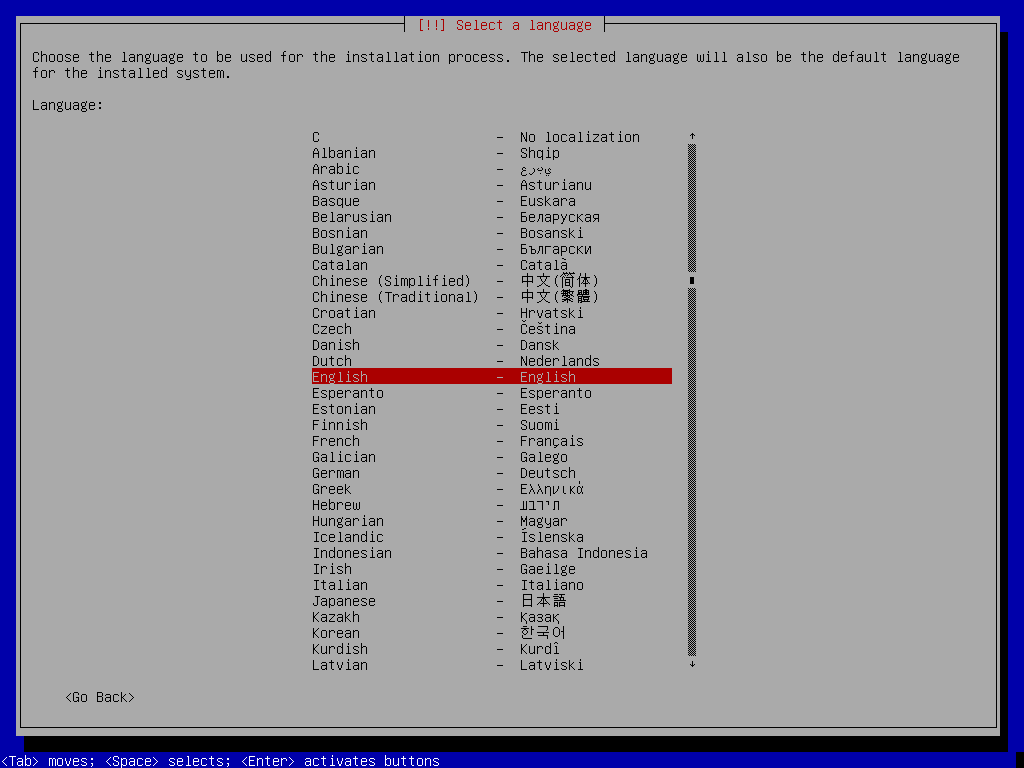
\includegraphics[width=\textwidth,natwidth=1024,natheight=768]{image201607/installer_console1.png} \\
	  Main Console (Alt-F1)
    \end{center}
    \column{0.5\textwidth}
    \begin{center}
      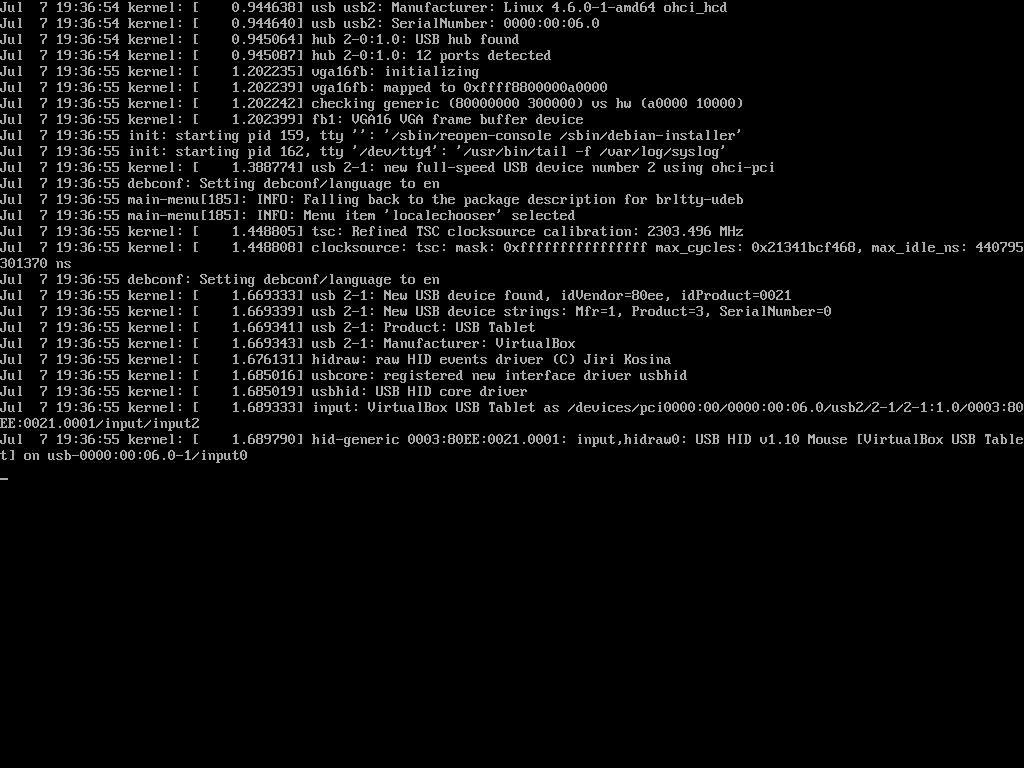
\includegraphics[width=\textwidth,natwidth=1024,natheight=768]{image201607/installer_console4.png} \\
	  Log Console (Alt-F4)
    \end{center}
  \end{columns}}

  \only<2>{
  For embedded device, serial console or SSH is used to install,
  so there's no way to switch console by Alt-F[Number].
  We have to go \textless Back\textgreater, and use command line shell from menu.
  \begin{center}
    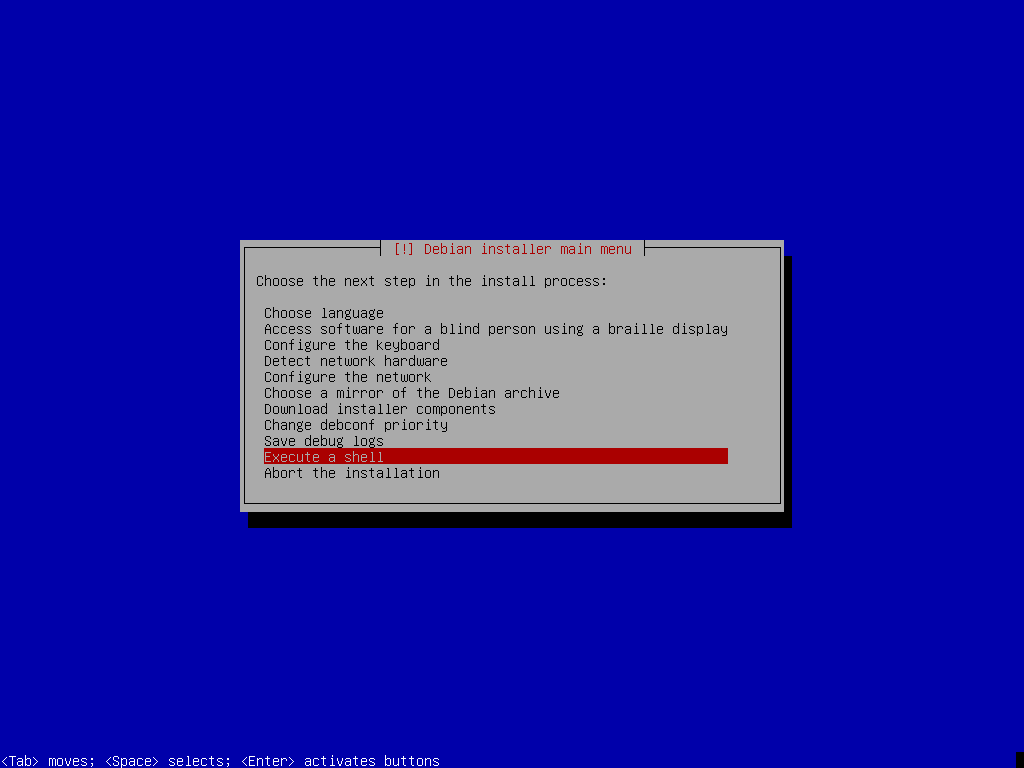
\includegraphics[width=\textwidth*4/5,natwidth=1024,natheight=768]{image201607/installer_shell.png}
  \end{center}
  }
\end{frame}


\section{Add screen support for D-I}

\subsection{Action Item List}
\begin{frame}{Action Item List}
  \begin{itemize}
  \item udeb support for all necessary packages and its dependencies
  \note[item]{This is not only for GNU/Screen support. If we want to add any new feature to D-I, it's required to have the same udeb support.}
  \item Add udeb to D-I image build
  \item Start/Resume GNU/Screen in D-I
  \end{itemize}
\end{frame}

\subsection{udeb Support for Packages}
\begin{frame}{udeb Support for Packages \only<2>{\small (cont.)}}
  \only<1>{
  \begin{itemize}
  \item Add udeb binary for GNU/Screen and it's dependencies.
  \note{First things first, all packages, to be included into the installer, need to be in udeb format.}
  \item It's in each package's debian/control
  \note{Usually it just need to add a few lines to each package in debian/control, and copy another a few lines to debian/\textless package\textgreater -udeb.install file.}
  \item Usually debian/\textless pkg\textgreater-udeb.install is the same as debian/\textless pkg\textgreater.install. Remove non-related files if any.
  \item Submit patch, and ask each package maintainers' help.
    \begin{itemize}
    \item Usually DM can upload to archive without sponsoring.
    \item However, for adding udeb case, unfortunately we have to find a DD to sponsor the upload because we add a new package (udeb).
	\item Due to the same reason, we also need to wait for approval from ftp-master (NEW queue)
    \end{itemize}
  \end{itemize}}

  \only<2>{
  \begin{itemize}
  \item Action Item:
    \begin{itemize}
	\item audit (libaudit1-udeb \& libaudit-common-udeb): BTS\#819358\footnote{\url{https://bugs.debian.org/819358}}
	\item pam (libpam0g): BTS\#819359\footnote{\url{https://bugs.debian.org/819359}}
	\item ncurses (libtinfo5-udeb): BTS\#819397\footnote{\url{https://bugs.debian.org/819397}}
	\item screen (screen-udeb): BTS\#819988\footnote{\url{https://bugs.debian.org/819988}}
    \end{itemize}
  \item Besides, we also need a proper ".screenrc" profile to emulate D-I on common PC with 4 active console.
    \begin{itemize}
    \item This change is included together with the upload of screen-udeb BTS\#819988\footnotemark[1]
    \end{itemize}
  \end{itemize}}
\end{frame}

\subsection{Add udeb to D-I image build}
\begin{frame}{Add udeb to D-I image build}
  \begin{itemize}
  \item Before we can invoke screen command within D-I environment, screen-udeb and it's dependency package is required to be included in the image.
  \item The package list of each D-I image is managed by d-i/debian-installer.git\footnote{\url{https://anonscm.debian.org/cgit/d-i/debian-installer.git}} repository.
    \begin{itemize}
	\item add "screen-udeb" to related Arch/Flavour of echo image: build/pkg-lists\footnote{\tiny\url{https://anonscm.debian.org/cgit/d-i/debian-installer.git/tree/build/pkg-lists}}
    \item Some image-size sensitive platform, such as armel/orion5x/qnap, can be excluded to avoid problem
    \end{itemize}
  \end{itemize}
\end{frame}

\subsection{Start/Resume GNU/Screen in D-I}
\begin{frame}{Start/Resume GNU/Screen in D-I}
  \begin{itemize}
  \item Suppose binaries are already in place, so we can hack the scripts to invoke GNU/screen when D-I starts.
  \item The logic is that resume previous screen session if possible, or we just start a new one.
  \item D-I boot scripts are mainly managed by d-i/rootskel.git\footnote{\url{https://anonscm.debian.org/cgit/d-i/rootskel.git}} repository.
  \end{itemize}
\end{frame}


\section{Progress Updates}

\begin{frame}{Progress Updates}
  \begin{itemize}
  \item I started from posting RFC to mailing-list to hear the voice from other developers and users, on February 20th, 2016\footnote{\tiny\url{https://lists.debian.org/debian-boot/2016/02/msg00547.html}}
  \item udeb support for all necessary packages and its dependencies
    \begin{itemize}
    \item audit (libaudit1-udeb \& libaudit-common-udeb) BTS\sout{\#819358}\footnote{\tiny\url{https://bugs.debian.org/819358}}: \alert{Done}\footnote{\tiny Thanks to Laurent Bigonville for his idea to build screen-udeb with less dependency, this udeb is not necessary anymore.}
	\item pam (libpam0g-udeb) BTS\sout{\#819359}\footnote{\tiny\url{https://bugs.debian.org/819359}}: \alert{Done}\footnotemark[2]
	\item ncurses (libninfo5-udeb): BTS\sout{\#819397}\footnote{\tiny\url{https://bugs.debian.org/819397}}: \alert{Uploaded} two weeks ago
	\item screen (screen-udeb) BTS\sout{\#819988}\footnote{\tiny\url{https://bugs.debian.org/819988}}: \alert{Uploaded} two weeks ago
    \end{itemize}
  \item Add udeb to D-I image build: \alert{Commit pushed} after D-I Stretch Alpha 7, so you can test D-I Daily\footnote{\tiny\url{https://d-i.debian.org/daily-images}}
  \item Start/Resume GNU/Screen in D-I: \alert{Done}\footnote{\tiny\url{https://anonscm.debian.org/cgit/d-i/rootskel.git/tree/src/sbin/debian-installer}}
  \end{itemize}
\end{frame}


\section{Devices will be Benefit}
\begin{frame}{Devices will be Benefit}
  \begin{itemize}
  \item Devices install via serial console, e.g. some ARM boards, and Sparc64 machine
  \item Devices install via SSH, e.g. some ARM boards, Mainframe s390/s390x
  \item Headless PC
  \end{itemize}
\end{frame}


\section{Credit}
\begin{frame}{Credit}
  \begin{itemize}
  \item Encouragement through early RFC stage
  \item Various help on udeb support
  \end{itemize}
\end{frame}

{\SWIRLBGhi
\begin{frame}{}
  \begin{center}
    \vfill \vfill
    {\LARGE Thanks for coming!}
    \vfill \vfill
    {\huge Any question or comment would be appreciated.}
    \vfill
    Roger Shimizu \\
    \texttt{rogershimizu@gmail.com} \\
    \url{https://wiki.debian.org/RogerShimizu}
  \end{center}
  \vfill \vfill
  {\tiny
    \begin{center}
      \begin{tabular}{l@{\hspace{1em}}l}
        \multicolumn{2}{l}{about the slides:} \\
        template from
        & \url{http://git.upsilon.cc/?p=talks.git} \\
        copyright \copyright ~ 2014 & Stefano Zacchiroli \\
        license
        & \href{http://creativecommons.org/licenses/by-sa/4.0/}{CC BY-SA 4.0 ---
          Creative Commons Attribution-ShareAlike 4.0} \\
      \end{tabular}
    \end{center}}
\end{frame}
}

\end{document}
